\chapter{Data Store}\label{ch:ch6label}

			Data store component can be considered as repository to store and manage the collection of information used in application. Generally data store can be classified as database in which data is stored in organised manner so that it can be easily accessed, managed and updated. For each application the database is designed according to the business logics and entities such that the data can be interpreted by components for the future use. The database management system(DBMS) is a system software used for creating and managing the databases. DBMS serves as an interface between database and the user or application programs, ensuring that data is consistently organized remains easily accessible. 
			
			Database can be categorised into different types on basis of the  structure of the stored data and the functionality.

\section{Relational Database} 

                 Relation database organises data into one or more tables which is formally described and organised according to the relational model . Each row in the table which is also called as record is a set of values related with each other in some way and a unique key identifying each row. Its focus is to implement simple CRUD - create, Read, update and Delete functionality. Each row represents an object and information about object.A relationship is established among the tables based on the interaction between them  which is derived from business logics of the application. Currently Mysql , PostgreSql,SQLite and Oracle are the popular RDBMS used for applications.  A connection is established between the application server and the database server using drivers. All the dbms has its own driver which provides API that defines how a client may access a database. Unlike database that exit in server side, SQLite is a in-memory embedded software used in client storage in the apllication such as web browser, mobile client etc.SQLite reads and writes directly to ordinary disk files. A complete SQL database with multiple tables, indices, triggers, and views, is contained in a single disk file. The database file format is cross-platform. These features make SQLite a popular choice as an Application File Format.  Basically  SQLite strive to provide local data storage for individual applications and device. But Mysql , PostgreSql and Oracle are Client/server SQL database engines aims at providing a shared repository of enterprise data.  
                   
                  
\begin{description}
  \item[$\bullet$] {\bfseries Connection Establishment:} Mysql , PostgreSql and Oracle are separate process running in the machine. Back end of the applications establishes connectivity with these DBMS using dedicated drivers API. But SQLite library is imported into the client side of an application and its functionality is called through function calls which is reduce latency in database access as SQLite doesn't have separate server process. Because function call within a single process is more efficient than inter-process communication.  
  \item[$\bullet$] {\bfseries Access Control:} To use databases in client-server systems, the connection establishment requires a user authentication and user based authorization service.But SQLite doesn’t require any authorization or authentication.Access control of SQLite is based on the file system permissions given to the database file itself. 
  \item[$\bullet$] {\bfseries Concurrent Access :} As client server database model focus on shared memory, it allows multiple user making it highly concurrent. For example MySQL with InnoDB storage engine does row level locking to support simultaneous write access by multiple sessions. MySQL with MyISAM storage engine does table level locking allowing single session to update tables at a time. But this can be alter to multi user by changing the concurrent\_insert system variable. SQLite design grants lock to the entire databases file during writing allowing concurrent read and sequential writes.  
\end{description}  
                 
\subsection{Usage}

\section{Mobile Database}

			Mobile application can have a centralized database which is connected to mobile over network and a database actually stored in the  mobile. Mobile device prefer database replication which means frequent retrieval of data from a centralised database and store it in the local database in the mobile.But bandwidth usage must be taken into consideration. Mobile client database contains a subset of data stored in the centralised database. Data synchronization is important to maintain the integrity between mobile server and mobile client. In some application, Queues are used to manage the information for synchronization.Most of the case, synchronization is asynchronous and the change propagation is not immediate. The best known mobile database for android and iOS is SQLite. But SQLite use complex schemas for data storage and access as it is relational database which impacts the user experience. Since SQLite doesn't have a inbuilt sync functionality, the sync code is self implemented which is considered to time consuming.   
			
			 

\subsection{Couchbase Mobile}

		Couchbase mobile is the first NoSQL JSON database that offers full flexibility of NoSQL to mobile.It is designed to provide fast and consistent access to data offline or online. Couchbase mobile consist of three components:i) 

\begin{figure}[!htb]
  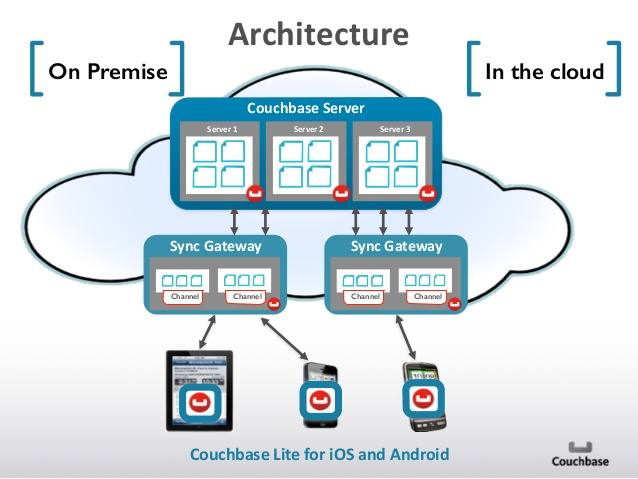
\includegraphics[width=\linewidth]{figures/Couchbase-Mobile-IOT-Database.jpg}
	 \caption{Couchbase Mobile Architecture}
  \label{fig: Couchbase Mobile Architecture}
\end{figure}			

		
\begin{description}
  \item[$\bullet$] {\bfseries Couchbase Lite:} Couchbase Lite is an lightweight embedded full featured JSON  document based and schemaless database on the device. It has APIs for Android,iOS and Rest along with integration support in popular cross-platform tools such as Phonegap and Xamarin. It includes features like peer-to-peer replication along with authorization by connecting with other mobile device running Couchbase Lite as its local storage and sync data with them after determining the document is replicated for that user.
 
    \item[$\bullet$] {\bfseries Couchbase Sync Gateway:} This component handles a two-way change synchronization between JSON store in Couchbase Server and Couchbase Lite.It  provides feature like routing required data to users avoid frequent network API calls, plug-in authentication, change validation and access control. 

  \item[$\bullet$] {\bfseries Couchbase Server:}	The NoSQL database that resides in the backend with elastic scalability and consistent high performance.
  
\end{description}


\subsection{Realm}

		Realm is a open source library launched in 2014 which can be integrated with the mobile application to store and query data. Realm introduced many features which made it appear as a replacement for SQLite.  

\begin{description}
  \item[$\bullet$] In this database , data is exposed as objects directly incorporating object relationships avoiding the need for ORM. At the same time, it remains extremely memory efficient. 
   \item[$\bullet$] It includes full ACID transactions default and an object schema is created directly driving from object definition.
   \item[$\bullet$] Unlike SQLite , Realm database are safe across threads making it highly concurrent when there is a burst of asynchronous task .  
\end{description}  


\section{Key - Value Database}

			Key-Value database is considered to be a simplest way storing data in the form of key-value pair and retrieving data based on key value. An advanced form of key-value store introduces the sorting of keys which enables an ordered processing of keys. Key-value database is also known as NoSQL databases. Key-Value store works differently when compared to relational database and it addresses several issues which relational database didn't address. Relational database 

\begin{description}
	\item[$\bullet$] Relational databases expects the schemas to be pre-defined which is poorly suited for agile development approaches as the schemas changes as the feature evolves.
	
\end{description}			
			
		
			
\subsection{Redis}
\subsection{Oracle NoSQL}
\subsection{MongoDB}

\section{Graph Database}

\subsection{Neo4j}
\subsection{Titan}







\section{In - Memory Database}

\subsection{Redis}
\subsection{Aerospike}

\section{Cloud Storage}

\subsection{Amazon S3}
\subsection{Amazon EBS}
\subsection{Google Cloud Storage}